\documentclass[a4paper,11pt]{report}
\usepackage[T1]{fontenc}
\usepackage[utf8]{inputenc}
\usepackage[francais]{babel}
\usepackage[babel=true,kerning=true]{microtype}
\usepackage[usenames,dvipsnames,svgnames,table]{xcolor}
\usepackage[colorlinks,linkcolor={blue!30!black},citecolor={blue!50!black},urlcolor={blue!80!black}]{hyperref}
\usepackage{amsmath,amsfonts,amssymb,array,graphicx,caption,lmodern,subcaption,tikz,url,xspace,wrapfig}
\usepackage{textcomp,rotating,epic,pdfpages,listings,diagbox,multirow,float}
\usepackage{pgfplots}
\pgfplotsset{width=7cm,compat=1.8}

\usepackage[top=25mm,bottom=25mm,left=25mm,right=25mm]{geometry}

\parskip=6pt % adds vertical space between paragraphs

\begin{document}

\pagenumbering{gobble}  % Pas de numérotation
\begin{titlepage}
    \vspace*{50px}
    
\includegraphics[height=80px]{Images/logo_phelma.pdf}
    \vspace*{-80px}
\begin{flushright}
%     \vspace*{60px}
    
\includegraphics[height=65px]{Images/CIME.jpg}
\end{flushright}

\vspace*{2cm}

\begin{center}
\rule{\linewidth}{0.5mm}\\[0.4cm]
{\huge{\bfseries Compte Rendu}\\[0.4cm]
\textsc{TP Simulation électronique}\\[0.4cm]}
\rule{\linewidth}{0.5mm}\\[0.5cm]

\LARGE{\textsc{Nicolas Paillet, Félix Piédallu \& Giulia Rizzo}}\\[0.7cm]
\large{\textsc{2015-2016}}\\[2cm]

\Large{~}\\[1cm]
% 
\includegraphics[width=0.4\textwidth]{Images/CIME.jpg}\\[1cm]
%
 \large{Encadrant : Marco Pala}\\[2cm]
%

\end{center}
\end{titlepage}

\tableofcontents        % Table des matières avec liens, générée automatiquement.
\newpage
\pagenumbering{arabic}  % Numérotation de retour !


\chapter*{Introduction}
\addcontentsline{toc}{chapter}{Introduction}
La fabrication de composants microélectroniques devient, lorsqu'on diminue la dimension, de plus en plus critique en terme de qualité. En effet, on va être sensibles à différents effets qui vont s'accentuer à faible dimension :
\begin{itemize}
    \item Les courants de fuite par la grille, qui s'accentuent à faible dimension par effet tunnel (lorsque l'épaisseur d'oxyde passe en dessous de 1,2nm)
    \item Les effets de canaux courts qui apparaissent lorsque la largeur de la grille diminue.
\end{itemize}

De plus, plus un composant est petit, plus la précision relative de fabrication va diminuer : les dimensions vont perdre en précisions, tandis que l'implantation et la diffusion de dopants dans le canal va apporter des processus aléatoires supplémentaires, à des échelles comparables aux dimensions des composants.

Pourtant, un processeur nécessite d'avoir des milliards de transistors de performances constantes, notamment une tension de seuil qui devra être la plus constante possible sur l'ensemble des transistors.

L'industrie microélectronique nécessite donc de caractériser parfaitement les transistors fabriqués. Le but de ce TP est donc de nous familiariser avec les techniques de caractérisation électronique, ainsi que de nous fournir un aperçu des performances des différentes technologies de transistors.

Nous avons à disposition des transistors BULK et FDSOI, de dimensions de grilles entre $30nm$ et $10\mu m$.


\chapter{Rappels des équations}

\chapter{Mesure de la tension de seuil}
La tension de seuil est la caractéristique principale de fonctionnement du transistor. Elle déterminera la consommation du dispositif, ainsi que sa performance en terme de fréquence de fonctionnement. Il est donc nécessaire de caractériser correctement cette tension.

Notamment, la tension de seuil doit être un paramètre constant dans une production industrielle.

\section{Méthode de la transconductance}
Cette méthode repose sur la caractéristique $I_d$ en fonction de $V_g$. En effet, ce tracé permet de déterminer assez facilement $V_T$. Cependant, une méthode uniquement visuelle n'est pas systématique et fortement dépendante de l'opérateur.

On peut alors calculer la dérivée de $I_d(V_g)$ ; la tangente à $I_d(V_g)$ dont la pente est maximale croise 0 en $V_T$. Cette méthode est beaucoup plus adaptée à une caractérisation fiable, automatisée et constante.


%TODO schéma graphe

\subsection{Transistor Bulk}
\begin{figure}
    \begin{center}
        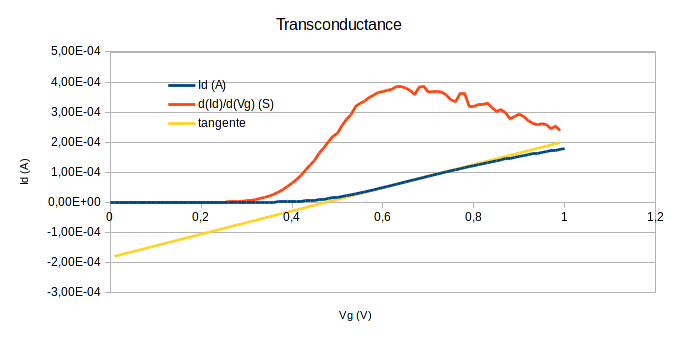
\includegraphics[width=\textwidth]{Images/Bulk40-Transconductance}
        \caption{Transconductance du transistor Bulk, $l=40\mu m$}
        \label{fig:}
    \end{center}
\end{figure}
%TODO résultats

\subsection{Transistor FDSOI}
\begin{figure}
    \begin{center}
        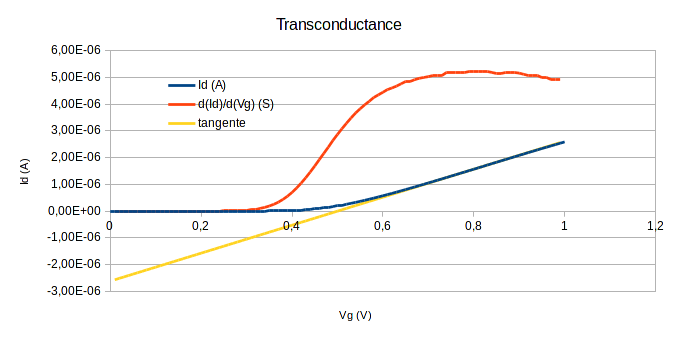
\includegraphics[width=\textwidth]{Images/FD1-10-Transconductance}
        \caption{Transconductance du transistor FDSOI, $l=10\mu m$}
        \label{fig:}
    \end{center}
\end{figure}
%TODO graphe
\noindent On obtient ainsi le gain du transistor \[\beta=G_m=341\mu S\] Ce maximum est atteint pour $V_G=670mV$.
%TODO graphe tangente

Le tracé de la tangente nous donne ainsi $V_T=450mV$.

\section{Méthode de la fonction Y}
On peut également utiliser une méthode différente pour déterminer $V_T$, à l'aide d'une fonction Y, définie par :
\[Y(V_g)=\dfrac{I_d(V_g)}{\sqrt{g_m(V_g)}}\]

Cette fonction est linéaire après le seuil, on peut alors approximer asymptotiquement plus précisément. On obtient alors $V_T$.
\subsection{Transistor Bulk}
%TODO graphes
\subsection{Transistor FDSOI}
%TODO graphes
%TODO résultats
\section{Méthode du courant constant}
A $V_d$ fort il n'est plus possible de trouver grâce à la méthode de la transconductance. On utilise alors une méthode dite du courant constant. Elle consiste à trouver un courant de seuil $I_{d_{TH}}$ pour $V_d$ faible, qui correspond au courant à $V_T$, puis de considérer la relation : \[I_{d_{TH}}=I_{d_{DN}}\cdot\dfrac{W}{L}\]

$I_{d_{DN}}$ est un paramètre arbitraire, un critère, réutilisable qui permet de calculer $V_T$ pour plusieurs transistors.

\subsection{Transistor FDSOI}
%TODO graphe

%TODO calculs

\chapter{Mesure du DIBL}
Le DIBL est également important à connaître %+blabla
On peut le calculer à partir des données précedentes.
%TODO calculs
On peut vérifier ces calculs en regardant la cours en log.
%TODO graphe
On peut également voir l'effet du DIBL en traçant des caractéristiques $I_d(V_d)$.
%TODO graphe 

\chapter{Comparaison des architectures}

\chapter*{Conclusion}
\addcontentsline{toc}{chapter}{Conclusion}

Ça marche. %Mais il y a des cons promis.


















\end{document}
